\documentclass[11pt,a4paper]{article}
\usepackage[utf8]{inputenc}
\usepackage[T1]{fontenc}
\usepackage{amsmath,amsfonts,amssymb}
\usepackage{apacite}
\usepackage{natbib}
\usepackage{graphicx}
\usepackage{booktabs}
\usepackage{threeparttable}
\usepackage{url}
\usepackage{hyperref}
\usepackage[margin=2.5cm]{geometry}
\usepackage{setspace}
\onehalfspacing

\newcommand{\Var}{\text{Var}}
\newcommand{\Cov}{\text{Cov}}

% Define \sym command for significance stars from esttab
\newcommand{\sym}[1]{{#1}}

\title{Estimating the Value of CEOs in Privately Held Businesses\thanks{Project no. 144193 has been implemented with the support provided by the Ministry of Culture and Innovation of Hungary from the National Research, Development and Innovation Fund, financed under the KKP\_22 funding scheme. This project was funded by the European Research Council (ERC Advanced Grant agreement number 101097789). The views expressed in this research are those of the authors and do not necessarily reflect the official view of the European Union or the European Research Council. \emph{Author contributions:} Conceptualization and study design: Koren, Orbán and Telegdy. Data curation, integration and quality assurance: Szilágyi and Vereckei. Statistical analysis: Koren and Telegdy. Writing the original draft: Koren. Review and editing: Koren, Orbán, Szilágyi, Telegdy and Vereckei. \emph{AI disclosure:} Claude Sonnet 4 was used to write and edit the research code and to format the manuscript (such as editing tables, figures, references, creating summaries). All code and text generated by AI tools were reviewed and edited by the authors. All authors have read and agreed to the published version of the manuscript. \emph{Data availability statement:} The data underlying this article cannot be shared publicly due to privacy and licensing restrictions. The replication package is available at \url{https://github.com/korenmiklos/ceo-value}.}}

\author{Miklós Koren\thanks{Central European University, HUN-REN Centre for Economic and Regional Studies, CEPR and CESifo. E-mail: korenm@ceu.edu} \\
        Krisztina Orbán\thanks{Monash University.} \\
        Bálint Szilágyi\thanks{HUN-REN Centre for Economic and Regional Studies.} \\
        Álmos Telegdy\thanks{Corvinus University of Budapest.} \\
        András Vereckei\thanks{HUN-REN Centre for Economic and Regional Studies, Institute of Economics.}}

\date{\today}

\begin{document}

\maketitle

\begin{abstract}
We estimate CEO value in private firms using Hungarian administrative data covering over one million firms and CEOs from 1992-2022. Our model separates owner-controlled inputs (capital, location) from CEO-controlled inputs (labor, materials). We introduce a placebo-controlled event study comparing actual CEO transitions to randomly assigned fake transitions in stable firms. Raw estimates suggest [[raw CEO effect]] percent performance differences between good and bad CEOs, but [[placebo effect]] percent is mechanical noise. The true causal effect is [[true CEO effect]] percent—only [[true effect as percent of raw]] percent of the raw correlation. Three-quarters of apparent CEO variation is spurious, explaining weak results in studies using manager fixed effects as explanatory variables.
\end{abstract}

\textbf{Keywords:} CEO value, private firms, productivity

\textbf{JEL Classification:} [To be added]

\newpage

\section{Introduction}

What is the value of CEOs to firm performance? A large literature documents that management matters for productivity, whether through consulting interventions that improve practices \citep{bloom2013does}, training programs that build capabilities, or leadership changes that reshape organizations \citep{Bertrand2003-io}. Event studies around CEO changes find mixed evidence, with some documenting substantial effects \citep{bennedsen2020ceos, metcalfe2023managers} while others find more modest impacts. Yet this evidence comes overwhelmingly from publicly traded firms in developed economies, where governance structures, data availability, and institutional contexts differ markedly from the vast majority of businesses worldwide. Understanding CEO effects in privately held firms—which employ most workers and generate most economic activity—remains a critical gap in our knowledge of what drives firm productivity.

Private firms differ from their public counterparts in three fundamental ways that complicate the measurement of CEO value. First, data limitations are severe: private firms disclose little about executive compensation, strategic decisions, or even basic financial performance beyond statutory requirements. Second, ownership concentration gives owners direct control over strategic choices, creating a division of decision rights that blurs the attribution of outcomes to CEOs versus owners \citep{fama1983separation, jensen1976theory, burkart2003family}. Third, private firms are typically smaller with shorter histories, making their performance data substantially noisier than that of established public companies. These differences are not merely technical complications—they fundamentally alter how we should model and measure managerial contributions to firm performance.

We address these challenges through three contributions. First, we develop a model that explicitly accounts for the division of control between owners who set fixed inputs (capital, location, industry) and CEOs who optimize variable inputs (labor, materials). This framework clarifies what CEOs can and cannot affect, enabling cleaner identification of their contribution. Second, we assemble comprehensive administrative data covering the universe of Hungarian firms and their CEO networks over three decades (1992-2022), tracking over [[total firms]] firms and [[total CEOs]] CEOs through multiple business cycles and institutional regimes. Third, and most importantly, we introduce a placebo-controlled event study design that separates true CEO effects from the mechanical noise that contaminates fixed effects estimates when managers have short tenures.

Our headline result challenges conventional wisdom about CEO importance. The naive comparison suggests that firms hiring good CEOs outperform those hiring bad CEOs by [[raw CEO gap]] percent—a seemingly large effect consistent with the view that leadership quality is paramount. However, our placebo control reveals that [[placebo gap]] percent of this difference arises purely from noise in the estimation process, not from actual skill differences. The true causal effect of CEO quality is [[true CEO effect]] percent: economically meaningful and statistically significant, but only [[true as percent of raw]] percent of what raw correlations suggest. Put differently, three-quarters of the apparent variation in CEO quality is spurious.

This finding relates to but extends the literature on CEO effects in public firms. Studies of public companies find mixed evidence on CEO impact, with some documenting substantial effects on firm policies and performance \citep{Bertrand2003-io, bennedsen2020ceos} while others find more modest contributions \citep{fee2013managers}. The challenge of separating CEO effects from firm effects has long been recognized \citep{Bertrand2003-io}, leading to strategies using exogenous CEO departures \citep{bennedsen2020ceos} or industry shocks \citep{metcalfe2023managers}. Our placebo approach complements these methods by directly measuring and removing the noise component rather than relying on rare exogenous events.

Our work also connects to the broader literature on management practices and firm productivity. While randomized controlled trials demonstrate that management training and consulting can substantially improve firm performance \citep{bloom2013does}, these interventions typically change practices rather than people. The question of whether replacing managers generates similar gains remains contentious. Evidence from public sector organizations suggests modest manager effects \citep{fenizia2022managers, janke2024role}, while studies of family firms find larger impacts when professional managers replace family members \citep{bennedsen2007inside}. Our results for private firms fall between these extremes: CEOs matter, but less than simple correlations suggest.

Methodologically, our paper builds on the two-way fixed effects literature in labor economics that decomposes wages into worker and firm components \citep{Abowd1999Econometrica, Card2018JoLE}. These studies face similar challenges from limited mobility creating small-sample bias \citep{andrews2008high} and have developed bias-correction methods \citep{Bonhomme2023-dx, gaure2014correlation}. We adapt this framework to the CEO-firm setting but add the crucial innovation of placebo controls to separate signal from noise. This approach is particularly valuable when studying managers who, unlike workers, typically have few observations per individual, making traditional bias-correction methods less effective.

\section{Conceptual Framework}

We develop a framework to measure CEO value in privately held firms where owners retain control over strategic decisions while delegating operational choices to managers. This division of decision rights, common in private businesses, has important implications for identifying manager effects.

\subsection{Production and Decision Rights}

Firms produce output using a Cobb-Douglas production function with both fixed and variable inputs. The production function for firm $i$ with manager $m$ at time $t$ is:
\begin{equation}\label{eq:production}
Q_{imt} = A_i Z_{m} \varepsilon_{it} K_{it}^\alpha L_{imt}^{\beta} M_{imt}^{\gamma}
\end{equation}
where $A_i$ represents time-invariant organizational capital (location, brand value, customer relationships), $Z_m$ captures manager skill, $\varepsilon_{it}$ is residual productivity, $K_{it}$ is physical capital, $L_{imt}$ is labor input, and $M_{imt}$ is intermediate input usage. 

In standard production function estimation, these three components would be combined into a single measure: $\Omega_{it} = A_i Z_m \varepsilon_{it}$, commonly called total factor productivity (TFP). Our framework decomposes TFP into firm-specific advantages ($A_i$), manager-specific skill ($Z_m$), and residual productivity shocks ($\varepsilon_{it}$) to identify the distinct contribution of managers. 

The key institutional feature we model is the separation of decision rights. Owners control physical capital investment ($K_{it}$) and organizational assets ($A_i$), including location choices, brand development, and CEO hiring decisions. Managers control labor hiring ($L_{imt}$), input purchasing ($M_{imt}$), and day-to-day operations. This separation reflects the reality of private businesses where owners maintain direct involvement in strategic decisions while delegating operational management.

With $\chi := 1 - \beta - \gamma$, the production function exhibits decreasing returns to scale in variable inputs ($\beta + \gamma < 1$), which pins down optimal firm size even under perfect competition. Fixed inputs $A_i$ and $Z_m$ create firm-specific and manager-specific advantages that generate economic rents.

\subsection{Optimal Input Choices and Revenue}

Managers maximize profit by choosing variable inputs optimally given the owner's fixed choices. Under sector-specific output price $P_{st}$, wage rate $W_{st}$, and material price $\varrho_{st}$, the first-order conditions yield closed-form solutions for optimal input demands. Substituting these back into the revenue function gives:
\begin{equation}\label{eq:revenue}
R_{imst} = (P_{st}A_i Z_m \varepsilon_{it})^{1/\chi}
K_{it}^{\alpha/\chi}
W_{st}^{-\beta/\chi}
\varrho_{st}^{-\gamma/\chi}
(1-\chi)^{(1-\chi)/\chi}
\end{equation}

Revenue increases in manager skill $Z_m$, organizational capital $A_i$, and physical capital $K_{it}$, while decreasing in input prices. The elasticity of revenue with respect to manager skill is $1/\chi > 1$, reflecting the leverage effect: better managers can scale up operations by hiring more variable inputs, amplifying their productivity advantage.

\subsection{Surplus and Manager Value}

The surplus accruing to fixed factors—what owners and managers ultimately care about—equals revenue minus payments to variable inputs:
\begin{equation}\label{eq:surplus}
S_{imst} = R_{imst} - W_{st}L_{imt} - \varrho_{st}M_{imt} = \chi R_{imst}
\end{equation}

Under Cobb-Douglas technology, surplus is a constant fraction $\chi$ of revenue. This proportionality means we can work directly with revenue throughout our analysis, simplifying estimation while preserving all economic insights. Taking logarithms of the revenue equation:
\begin{equation}\label{eq:log_revenue}
r_{imst} = C+\frac{\alpha}{\chi} k_{it} + \frac{1}{\chi} z_{m} + \frac{1}{\chi} a_i + \frac{1}{\chi} p_{st} + \frac{1}{\chi}\epsilon_{it} 
- \frac{\beta}{\chi} w_{st} - \frac{\gamma}{\chi} \rho_{st}
\end{equation}
where lowercase letters denote logarithms (e.g., $\epsilon_{it} = \log \varepsilon_{it}$) and $C$ is a constant.

The value of replacing manager $m$ with manager $m'$ at the same firm is:
\begin{equation}\label{eq:manager_value}
r_{im'st} - r_{imst} = \frac{1}{\chi}(z_{m'} - z_{m})
\end{equation}

Manager value equals the skill difference scaled by $1/\chi$. This scaling reflects the leverage effect: a 1\% increase in manager skill generates a $(1/\chi)\%$ increase in revenue.

\subsection{Empirical Specification}

To estimate manager effects from observational data, we substitute unobserved prices and organizational capital with fixed effects:
\begin{equation}\label{eq:empirical}
r_{imst} = \frac{\alpha}{\chi} k_{it} + \frac{1}{\chi}z_m + \lambda_i + \mu_{st} + \tilde{\epsilon}_{it}
\end{equation}
where $\lambda_i = a_i/\chi$ captures time-invariant firm characteristics, $\mu_{st}$ absorbs sector-time variation in prices, and $\tilde{\epsilon}_{it} = \epsilon_{it}/\chi$ is rescaled residual productivity.

The key identifying assumption is that residual productivity $\tilde{\epsilon}_{it}$ is uncorrelated with manager assignment conditional on firm and sector-time fixed effects. This allows manager skills and physical capital to be arbitrarily correlated with firm quality and market conditions—better firms may hire better managers and invest more. We only require that the residual variation in productivity is orthogonal to manager assignment.

\subsection{Challenges in Estimating Manager Effects}

Three challenges complicate the estimation of manager effects from equation \eqref{eq:empirical}:

First, residual productivity $\tilde{\epsilon}_{it}$ may correlate with manager changes if firms replace CEOs in response to productivity shocks. This reverse causality would bias estimates of manager effects.

Second, manager fixed effects are only identified for the connected set of firms and managers linked through mobility. Effects are measured relative to a reference group within each connected component, limiting comparability across components.

Third, and most importantly, estimated manager effects $\hat{z}_m$ include both true skill and averaged residual productivity: $\hat{z}_m = z_m + \bar{\epsilon}_{im}$ where $\bar{\epsilon}_{im}$ is the average $\tilde{\epsilon}_{it}$ during manager $m$'s tenure at firm $i$. When managers have short tenures, this noise component dominates the signal, making raw fixed effects unreliable measures of true skill.

Our placebo-controlled approach addresses these challenges by explicitly measuring and removing the noise component from estimated manager effects.

\section{Corporate Data from Hungary}

Hungary provides an ideal setting for studying CEO effects in private firms. The country offers complete administrative data coverage for all incorporated businesses with mandatory CEO registration, spanning over 30 years from the transition economy of the 1990s through EU accession in 2004 to the present. This comprehensive coverage enables us to track CEO careers across firms and construct the mobility networks necessary for identification.

\subsection{Data Sources}

Our analysis combines two administrative datasets. The firm registry, maintained by Hungarian corporate courts, contains legally mandated records on all company representatives—individuals authorized to act on behalf of firms in legal and business matters. These records include CEOs and other executives with signatory rights, tracked through a temporal database where each entry reflects representation status over specific time intervals. Updates occur not only when positions change but also when personal identifiers are modified or reporting standards evolve. The registry provides names, addresses, dates of birth (from 2010), and mother's names (from 1999), though numerical identifiers only exist from 2013 onward.

The balance sheet dataset contains annual financial reports for essentially all Hungarian firms required to file statements. This includes sales revenue, export revenue, employment counts, tangible and intangible assets, raw material and intermediate input costs, personnel expenses, and indicators for state and foreign ownership. The two datasets together cover [[total firms]] firms over [[total years]] years, yielding [[total firm-years]] firm-year observations before sample restrictions.

\subsection{Entity Resolution and CEO Identification}

Constructing a panel of CEOs requires resolving two fundamental questions: what constitutes a firm and who qualifies as a CEO. For firms, we track legal entities through time using tax identifiers, which remain relatively stable despite occasional reuse (approximately [[tax ID reuse percent]]\% of cases). Mergers and acquisitions create new entities in our framework—we follow individual legal entities rather than economic conglomerates.

Identifying individual CEOs poses greater challenges. Before 2013, no numerical identifiers existed, requiring entity resolution based on names, addresses, mother's names, and birthdates. We link records across these dimensions to create unique person identifiers, enabling tracking across firms and over time. The quality of matching improves substantially after 1999 (mother's names) and 2010 (birthdates), though even the 1990s data achieves reasonable coverage through careful name and address matching.

CEO identification within firms requires additional heuristics since job titles are inconsistently recorded. When explicit "managing director" titles exist (approximately [[managing director percent]]\% of cases), we use them directly. For remaining cases, we assume all representatives are CEOs if three or fewer exist at the firm. When more than three representatives are present, we assign CEO status based on continuity with previously identified CEOs. Time spans between appointments are often unclosed or non-contiguous, requiring imputation based on sequential information and assuming representatives remain active if their tenure includes June 21 of each year.

\subsection{Sample Restrictions}

We apply several restrictions to create a sample suitable for productivity analysis. First, we exclude mining and finance sectors due to their specialized accounting frameworks and regulatory environments. Second, we drop firms ever having more than [[max simultaneous CEOs]] simultaneous CEOs (removing [[dropped for multiple CEOs]] observations) to avoid complex governance structures that complicate identification. Third, we exclude firms with more than [[max CEO changes]] CEO changes over the sample period ([[dropped for excess changes]] observations) to reduce noise from potentially misclassified transitions. Fourth, we remove all state-owned enterprises, as their objectives and constraints differ fundamentally from private businesses.

Most importantly, we restrict attention to firms that at some point employ at least [[min employees]] workers. This filter removes [[percent dropped for size]] of observations but eliminates shell companies, tax optimization vehicles, and self-employment arrangements masquerading as corporations. The remaining firms represent genuine businesses with meaningful economic activity where management quality plausibly affects performance.

\subsection{CEO and Firm Characteristics}

The resulting sample contains distinctive patterns of CEO demographics and tenure. Among CEOs in our analysis sample, [[percent Hungarian names]]\% have Hungarian names (verified algorithmically), with only [[percent foreign names]]\% foreign. Gender identification among Hungarian-named CEOs reveals [[percent male]]\% male representation. Remarkably, [[percent founders]]\% of CEOs were present at their firm's founding, highlighting the prevalence of founder-managers in private businesses.

CEO mobility creates networks essential for fixed effects identification. Approximately [[percent multiple firms]]\% of CEOs manage multiple firms during the sample period, generating connections between firms. The largest connected component of the bipartite firm-CEO network contains [[connected component size]] managers and a comparable number of firms—roughly [[percent in component]]\% of all managers but representing a substantial share of economic activity. This connected component enables comparison of CEO effects within a common reference frame, though raises questions about representativeness we address in robustness checks.

\subsection{CEO Turnover Patterns}

CEO tenure exhibits substantial variation across firms. While [[percent single CEO firms]]\% of firms retain the same CEO throughout their observed lifetime, the remaining firms experience leadership transitions that enable identification. Among firm-years with CEO information, [[percent single CEO firm-years]]\% have single CEOs, [[percent two CEO firm-years]]\% have two, and [[percent multiple CEO firm-years]]\% have more (before our sample restrictions). CEO spell lengths follow approximately an exponential distribution with a [[annual hazard rate]]\% annual hazard rate, implying typical tenures of [[typical tenure range]] years.

To validate our placebo methodology, we verify that synthetically generated CEO transitions match actual patterns. Taking firms with stable leadership (same CEO for [[min stable tenure]]+ years), we randomly assign placebo transitions using the empirical hazard function. The resulting spell length distribution closely mirrors actual CEO changes: [[percent one year spells]]\% last one year, [[percent two year spells]]\% two years, declining thereafter. This similarity confirms that our placebo transitions capture realistic turnover dynamics while maintaining the crucial property that no actual skill change occurs.

\section{Estimation}

Our estimation proceeds in four steps: measuring the surplus share, estimating the revenue function, recovering manager fixed effects, and validating causality through event studies. Each step builds toward separating true CEO effects from the substantial noise that contaminates raw estimates.

\subsection{Step 1: Measuring the Surplus Share}

The parameter $\chi$—the share of surplus in revenue—determines how manager skill translates into firm performance. Under Cobb-Douglas technology, this share equals one minus the combined revenue shares of labor and materials. Following \citet{Gandhi2020-nu}, we measure $\chi$ directly from the data as:
\begin{equation}
\hat{\chi}_s = 1 - \frac{\sum_{i \in s}(W_{st}L_{it} + \varrho_{st}M_{it})}{\sum_{i \in s} R_{it}}
\end{equation}
where the summation runs over firms in sector $s$.

This approach yields sector-specific estimates of $\chi$. The $1/\chi$ scaling in our framework creates a leverage effect where manager skill is amplified in its impact on firm performance. Following \citet{Halpern2015-se} and \citet{Gandhi2020-nu}, we compute $\chi$ directly from the data as the complement of factor shares.

\subsection{Step 2: Estimating the Revenue Function}

With $\hat{\chi}$ measured, we estimate the revenue function to recover the capital elasticity and control for observable factors. Using lowercase letters for logarithms, the estimating equation is:
\begin{equation}
r_{imst} = \frac{\alpha}{\chi} k_{it} + \frac{1}{\chi}z_m + \lambda_i + \mu_{st} + \tilde{\epsilon}_{it}
\end{equation}
where $r_{imst} = \log R_{imst}$ is log revenue, $k_{it} = \log K_{it}$ is log capital, $\lambda_i$ captures firm fixed effects, $\mu_{st}$ are sector-year fixed effects, and $\tilde{\epsilon}_{it} = \epsilon_{it}/\chi$ is rescaled residual productivity.

In practice, we allow firm productivity to vary across CEOs by including firm-CEO fixed effects $\lambda_{im}$ rather than separate firm and manager effects. This captures the joint contribution of organizational capital and manager skill for each firm-manager pair. We also include controls for firm age, intangible asset presence, and foreign ownership, though these barely affect the capital coefficient.

The key assumptions are: (1) all firms within a sector face the same prices, (2) residual productivity $\tilde{\epsilon}_{it}$ is uncorrelated with owner and manager choices, and (3) owner and manager choices can be arbitrarily correlated with each other. Assumption (2) is critical—we do not require random manager assignment, only that the residual productivity after controlling for observables is orthogonal to CEO changes.

We estimate using OLS with high-dimensional fixed effects via \texttt{reghdfe} \citep{reghdfe}. The coefficient on log capital is $\hat{\alpha}/\hat{\chi}$, which we multiply by $\hat{\chi}$ to recover $\hat{\alpha}$.

\subsection{Step 3: Recovering Manager Fixed Effects}

After estimating the revenue function, we compute log total factor productivity by removing the contribution of capital from revenue:
\begin{equation}
\omega_{imst} = \hat{\chi} r_{imst} - \hat{\alpha} k_{it} - \hat{\mu}_{st} = z_m + a_i + \epsilon_{it}
\end{equation}

This measure of log TFP contains manager skill, firm effects, and residual productivity. Recall that in standard production function estimation, this entire term would be treated as a single TFP measure. Our decomposition separates the manager contribution from other sources of productivity.

To isolate manager effects, we remove the firm fixed effect by subtracting the firm average:
\begin{equation}
\Delta\omega_{imt} = \Delta z_{m_{it}} + \Delta\epsilon_{it}
\end{equation}
where $\Delta x_{it} := x_{it} - \frac{1}{N_i}\sum_{\tau} x_{i\tau}$ denotes the within-firm deviation.

When a firm changes CEOs, the change in log TFP captures both the true skill difference and accumulated noise. The noise component—the average of residual productivity shocks during each manager's tenure—can dominate the signal when tenures are short.

\subsubsection{Two-Way Fixed Effects in the Connected Component}

For broader comparisons across firms, we estimate a two-way fixed effects model:
\begin{equation}
\omega_{imst} = a_i + z_m + \epsilon_{it}
\end{equation}

This system is only identified within connected components—groups of firms and managers linked through mobility. Two managers can be compared if they worked at the same firm or connect through a chain of shared employment relationships. Our largest connected component contains [[connected component size]] managers, enabling meaningful comparisons within this network. Following \citet{Abowd1999Econometrica}, we normalize one manager's effect to zero and estimate via within-transformation.

\subsubsection{Three Identification Challenges}

First, residual productivity trends may correlate with manager changes (reverse causality). Firms might replace CEOs when $\epsilon_{it}$ declines, creating spurious negative effects for incoming managers. We do not need random mobility—manager quality can correlate with firm quality—but we require that residual productivity shocks are orthogonal to CEO transitions.

Second, firm and manager effects are only interpretable within their connected component. Effects measure relative differences from a baseline group, limiting cross-component comparisons.

Third, and most critically, estimated fixed effects contain substantial small-sample noise. With short CEO tenures, the averaged residual productivity $\bar{\epsilon}_{im}$ often overwhelms true skill differences. Instrumental variable approaches that rely on exogenous CEO removal (death, hospitalization) address reverse causality but exacerbate the small-sample problem by further restricting the data.

\subsection{Step 4: Placebo-Controlled Event Studies}

Our solution to the noise problem leverages a simple insight: when CEOs do not change, we still observe variation in log TFP driven purely by noise:
\begin{equation}
\Delta\omega_{imt} = \Delta\epsilon_{it}
\end{equation}

By applying the same estimation procedure to "non-changes," we can measure and filter out the noise component.

\subsubsection{Constructing Placebo Transitions}

We construct placebo CEO transitions in three steps. First, we estimate the time-varying hazard of actual CEO changes. Second, we identify firms with long CEO tenures (7+ years) where no actual change occurs. Third, we randomly assign placebo transitions to these stable firms using the estimated hazard function.

For instance, a firm with the same CEO from 1992-2000 might receive a placebo transition in 1996, artificially splitting the tenure into two pseudo-CEOs. The timing follows the empirical hazard, ensuring the mechanical noise properties—averaging residual productivity over varying tenure lengths—match between actual and placebo groups.

\subsubsection{Event Study Design}

We implement the event study around CEO transitions at time $g$, comparing actual changes (treatment) to placebo changes (control):
\begin{equation}
\omega_{imt} = a_i + \gamma_{t-g} + \epsilon_{it}
\end{equation}

The coefficients $\gamma_{t-g}$ capture the evolution of log TFP in event time, where $t-g \in \{-4, -3, -2, -1, 0, 1, 2, 3\}$ and we normalize $\gamma_{-1} = 0$.

Because both groups receive a "treatment" (actual or placebo), standard difference-in-differences fails. We adapt the \citet{Callaway2021JoLE} estimator for two treatment types using the \texttt{xt2treatments} package \citep{Koren2024xt2treatments}. The key innovation is precisely aligning transitions in event time—both actual and placebo changes occur at $t=0$—enabling clean comparison of dynamics.

\subsubsection{Separating Good from Bad CEOs}

To examine heterogeneity in CEO quality, we split actual transitions based on the incoming CEO's estimated fixed effect $\hat{z}_m$ from Step 3. CEOs with above-median $\hat{z}_m$ are classified as "good," those below as "bad."

This classification is noisy—"good" CEOs are partly lucky (positive $\epsilon$ draws), "bad" CEOs partly unlucky (negative $\epsilon$ draws). But this is precisely the bias our placebo control corrects. When we randomly split stable tenures and classify the resulting pseudo-CEOs as good or bad based on their averaged $\epsilon_{it}$, we generate the same mechanical selection bias without any true quality difference.

\subsubsection{The Placebo Correction in Practice}

The placebo control reveals the extent of noise contamination in estimated manager effects. The decomposition shows that a substantial portion of apparent CEO effects are spurious, explaining why studies using manager fixed effects as explanatory variables often find weak or inconsistent results—they are measuring mostly noise. Our placebo method provides a practical solution for future research: always benchmark against placebo transitions to isolate true effects from mechanical bias.

\section{Results}

\subsection{Surplus Share and Revenue Function Estimates}

Table \ref{tab:surplus_share} in the Appendix reports our estimates of the surplus share $\chi$ by industry. The estimates range from [[chi min]] to [[chi max]] across sectors, with wholesale, retail, and transport showing the lowest values and professional services showing the highest. These estimates imply that a 1\% increase in TFP increases revenue by [[revenue amplification range]] percent through the leverage effect of scaling variable inputs.

Table \ref{tab:revenue_function} presents the revenue function estimates. We include controls for log capital, firm age, presence of intangible assets, and foreign ownership, along with firm-CEO and sector-year fixed effects. The capital coefficient is precisely estimated at [[capital coefficient]] (standard error [[capital SE]]), consistent with capital's limited but significant role in private businesses. The intangible asset dummy shows a positive coefficient of [[intangible coefficient]], while foreign ownership contributes [[foreign coefficient]] to log revenue. Firm age exhibits diminishing returns with a coefficient of [[age coefficient]] on log age. These controls explain [[R-squared]] of the variation in log revenue. Additional robustness checks varying the control set and sample restrictions, reported in the Appendix, yield similar estimates.

\begin{table}[htbp]\centering
\def\sym#1{\ifmmode^{#1}\else\(^{#1}\)\fi}
\caption{Surplus Function Estimation Results}
\begin{tabular}{l*{6}{c}}
\toprule
                    &\multicolumn{1}{c}{(1)}&\multicolumn{1}{c}{(2)}&\multicolumn{1}{c}{(3)}&\multicolumn{1}{c}{(4)}&\multicolumn{1}{c}{(5)}&\multicolumn{1}{c}{(6)}\\
                    &\multicolumn{1}{c}{Revenue}&\multicolumn{1}{c}{EBITDA}&\multicolumn{1}{c}{Wagebill}&\multicolumn{1}{c}{Materials}&\multicolumn{1}{c}{Revenue}&\multicolumn{1}{c}{Revenue}\\
\midrule
Fixed assets (log)  &       0.272\sym{***}&       0.263\sym{***}&       0.251\sym{***}&       0.323\sym{***}&       0.260\sym{***}&       0.271\sym{***}\\
                    &     (0.002)         &     (0.002)         &     (0.002)         &     (0.002)         &     (0.002)         &     (0.034)         \\
\addlinespace
Has intangible assets&       0.140\sym{***}&       0.085\sym{***}&       0.155\sym{***}&       0.165\sym{***}&       0.135\sym{***}&       0.212\sym{**} \\
                    &     (0.004)         &     (0.005)         &     (0.004)         &     (0.005)         &     (0.004)         &     (0.089)         \\
\addlinespace
Foreign owned       &       0.051\sym{***}&       0.017         &       0.086\sym{***}&       0.044\sym{**} &       0.059\sym{***}&       0.167         \\
                    &     (0.015)         &     (0.017)         &     (0.015)         &     (0.019)         &     (0.015)         &     (0.238)         \\
\midrule
Observations        &     1169474         &      927037         &     1157713         &     1184973         &     1169474         &        4122         \\
\bottomrule
\multicolumn{7}{l}{\footnotesize Standard errors in parentheses}\\
\multicolumn{7}{l}{\footnotesize All models include firm-CEO-spell fixed effects and industry-year fixed effects. Outcome variables are}\\
\multicolumn{7}{l}{\footnotesize log-transformed. Models (5) and (6) include quadratic controls for firm age and CEO tenure.}\\
\multicolumn{7}{l}{\footnotesize Model (6) restricts to largest connected component.}\\
\multicolumn{7}{l}{\footnotesize \sym{*} \(p<0.10\), \sym{**} \(p<0.05\), \sym{***} \(p<0.01\)}\\
\end{tabular}
\end{table}


\subsection{Distribution of Manager Fixed Effects}

After removing the contribution of capital and other controls from revenue, we estimate manager fixed effects within the largest connected component. Figure \ref{fig:manager_distribution} shows the distribution of these estimated effects. The raw dispersion is substantial: the interquartile range spans [[IQR]] log points, suggesting that moving from a 25th percentile to a 75th percentile CEO would increase firm productivity by approximately [[raw IQR productivity difference]] percent. However, as we demonstrate below, most of this variation reflects noise rather than true skill differences.

\begin{figure}[htbp]
\centering
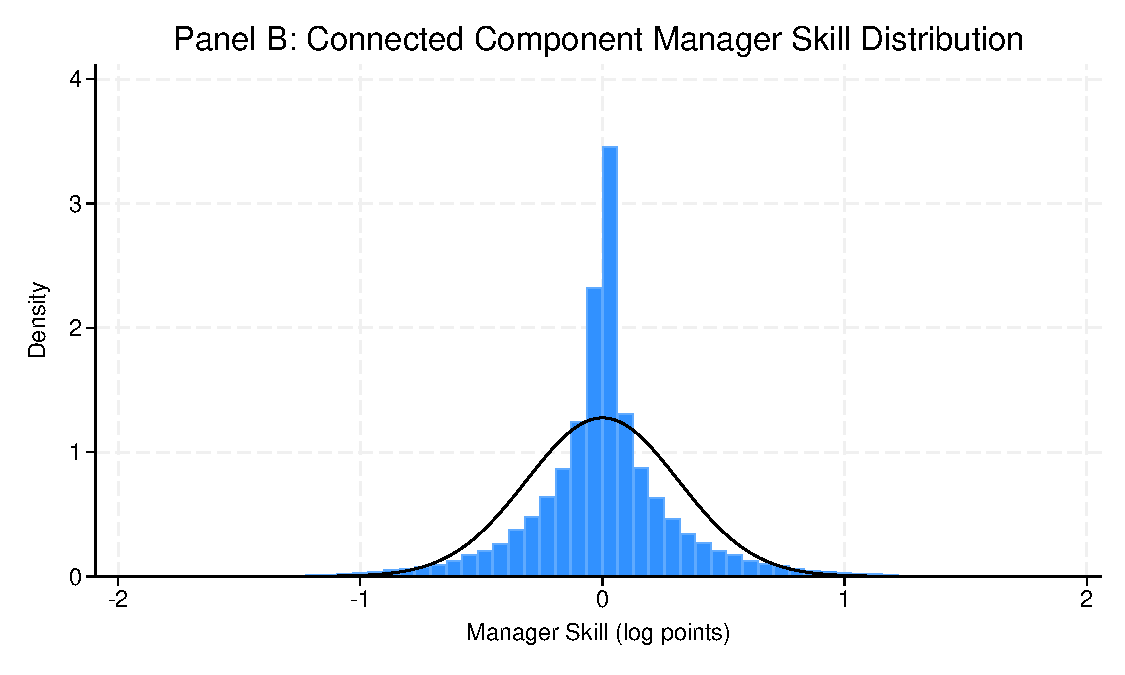
\includegraphics[width=0.8\textwidth]{figure/manager_skill_connected.pdf}
\caption{Distribution of Manager Fixed Effects in the Connected Component}
\label{fig:manager_distribution}
\end{figure}

\subsection{Event Study Evidence}

To examine the dynamics of firm performance around CEO transitions, we implement an event study analysis. Figure \ref{fig:event_study_combined} presents both the mean and variance of log TFP in event time, where year 0 marks the first year of the new CEO.

We examine variance alongside mean effects for a specific reason. Under our framework, if CEO changes are real and consequential, they should increase the cross-sectional variance of outcomes—some firms get better CEOs, others get worse ones. In contrast, pure noise or firm-specific trends would not systematically alter variance at the transition point.

\begin{figure}[htbp]
\centering
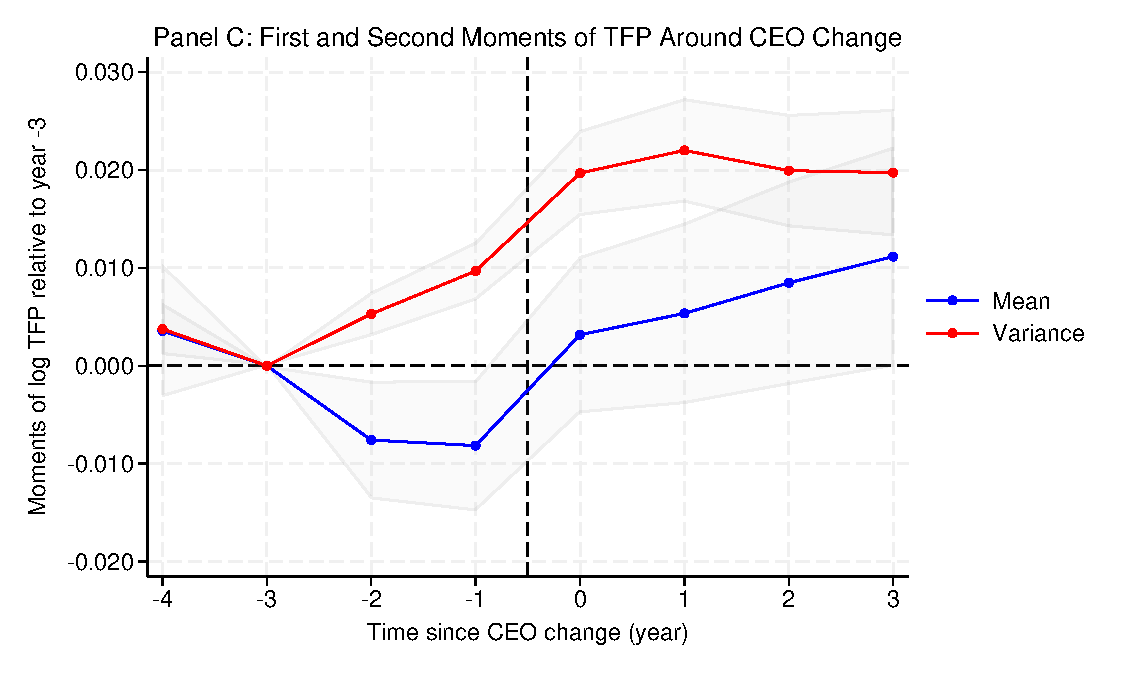
\includegraphics[width=0.8\textwidth]{figure/event_study_panel_c.pdf}
\caption{Mean and Variance of TFP Around CEO Transitions}
\label{fig:event_study_combined}
\end{figure}

The results reveal two key patterns. First, average TFP dips slightly in the two years before CEO change, declining by approximately [[pre-transition dip]] percent relative to year -3. This suggests firms experiencing performance difficulties are more likely to replace their CEOs, though the magnitude is modest. Second, and more importantly, the variance of TFP jumps sharply at the transition point, increasing by [[variance jump]] percent and remaining elevated thereafter. This variance increase is exactly what we would expect if CEO changes introduce real heterogeneity in managerial quality.

\subsection{Separating Good from Bad CEOs: Placebo-Controlled Estimates}

To quantify the causal effect of CEO quality, we split CEO transitions based on the incoming manager's estimated fixed effect. CEOs with above-median fixed effects are classified as "good," those below as "bad." We emphasize that this classification is based on noisy estimates that combine true skill with averaged residual productivity shocks.

Figure \ref{fig:event_study_split} presents the event study results for these two groups, comparing actual transitions to placebo transitions. The left panel shows firms hiring "good" CEOs, the right panel those hiring "bad" CEOs.

\begin{figure}[htbp]
\centering
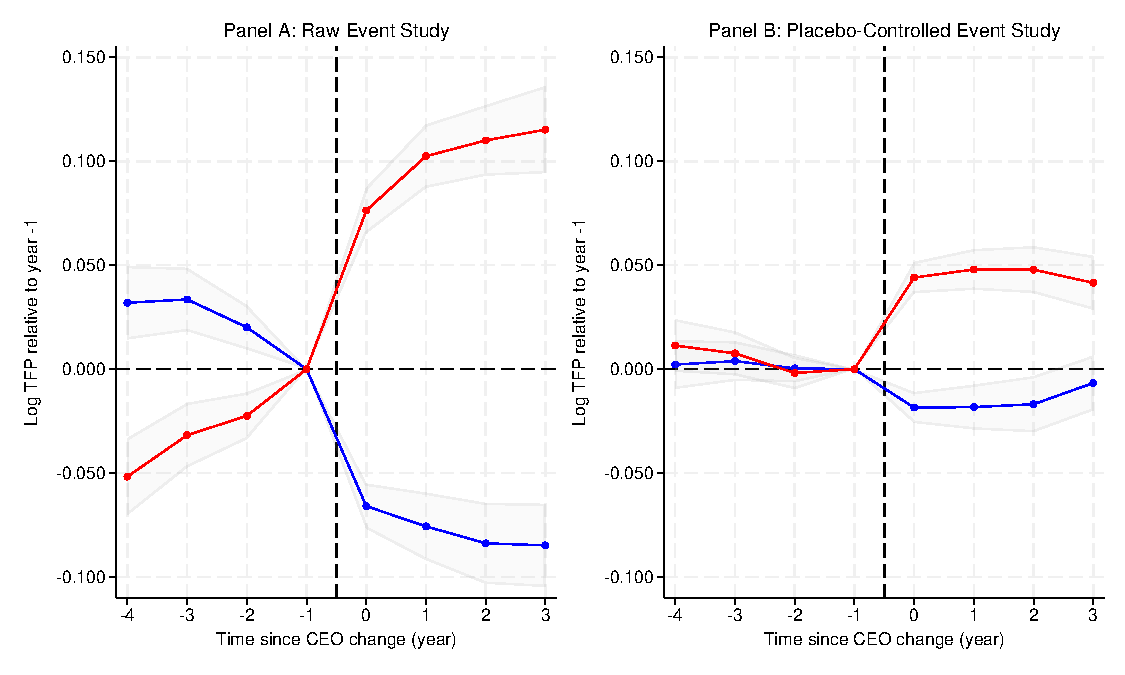
\includegraphics[width=\textwidth]{figure/event_study.pdf}
\caption{Event Study by CEO Quality: Actual vs Placebo Transitions}
\label{fig:event_study_split}
\end{figure}

Without the placebo control, we would conclude that good CEOs improve TFP by [[raw good CEO effect]] percent while bad CEOs reduce it by [[raw bad CEO effect]] percent, yielding a total gap of [[raw CEO gap]] percent. However, the placebo transitions—where no actual skill change occurs—generate effects of [[placebo good effect]] and [[placebo bad effect]] percent respectively, a gap of [[placebo gap]] percent driven purely by mechanical selection on noise.

Table \ref{tab:atet_manager} reports the average treatment effects on the treated (ATET), computed as the difference between actual and placebo effects. The true causal impact of hiring a good versus bad CEO is [[true CEO effect]] percent—statistically significant but only [[true as percent of raw]] percent of the raw correlation. This decomposition reveals that approximately [[percent noise]] percent of the apparent variation in CEO effects is spurious.

{
\def\sym#1{\ifmmode^{#1}\else\(^{#1}\)\fi}
\begin{tabular}{l*{2}{c}}
\hline\hline
                    &\multicolumn{1}{c}{(1)}&\multicolumn{1}{c}{(2)}\\
                    &\multicolumn{1}{c}{Wagebill (log)}&\multicolumn{1}{c}{Materials (log)}\\
\hline
Better CEO          &       0.055\sym{***}&       0.127\sym{***}\\
                    &     (0.013)         &     (0.013)         \\
\hline
Observations        &     1089713         &     1089713         \\
\hline\hline
\end{tabular}
}


\subsection{Effects on Different Outcomes}

Our model predicts that CEOs should primarily affect outcomes they control (labor, materials) rather than those controlled by owners (capital, organizational structure). Tables \ref{tab:atet_manager} and \ref{tab:atet_owner} test these predictions by examining various outcomes.

Good CEOs have immediate and substantial effects on manager-controlled variables. Log employment increases by [[employment effect]] percent, log materials by [[materials effect]] percent, and log revenue by [[revenue effect]] percent. These effects appear immediately in year 0 and persist throughout the post-period, consistent with new CEOs quickly adjusting operational scale.

{
\def\sym#1{\ifmmode^{#1}\else\(^{#1}\)\fi}
\begin{tabular}{l*{3}{c}}
\hline\hline
                    &\multicolumn{1}{c}{(1)}&\multicolumn{1}{c}{(2)}&\multicolumn{1}{c}{(3)}\\
                    &\multicolumn{1}{c}{Fixed assets (log)}&\multicolumn{1}{c}{Has intangible assets}&\multicolumn{1}{c}{Foreign owned}\\
\hline
Better CEO          &       0.054         &       0.056\sym{***}&       0.051\sym{***}\\
                    &     (0.078)         &     (0.020)         &     (0.013)         \\
\hline
Observations        &       81272         &       81272         &       81272         \\
\hline\hline
\end{tabular}
}


In contrast, owner-controlled variables show markedly different patterns. Fixed assets exhibit no significant change ([[capital effect]] percent, not statistically different from zero), validating our assumption that CEOs cannot independently alter capital stock. Foreign ownership probability increases gradually by [[foreign ownership effect]] percentage points, but only after year 2, suggesting this reflects owner decisions rather than CEO actions.

Intangible assets present an interesting intermediate case. Figure \ref{fig:intangibles} shows that the probability of reporting intangibles increases by [[intangible effect]] percentage points under good CEOs, but the effect builds gradually over three years rather than jumping immediately. This pattern suggests intangibles may reflect joint owner-CEO decisions or that successful CEOs earn greater owner trust over time.

\begin{figure}[htbp]
\centering
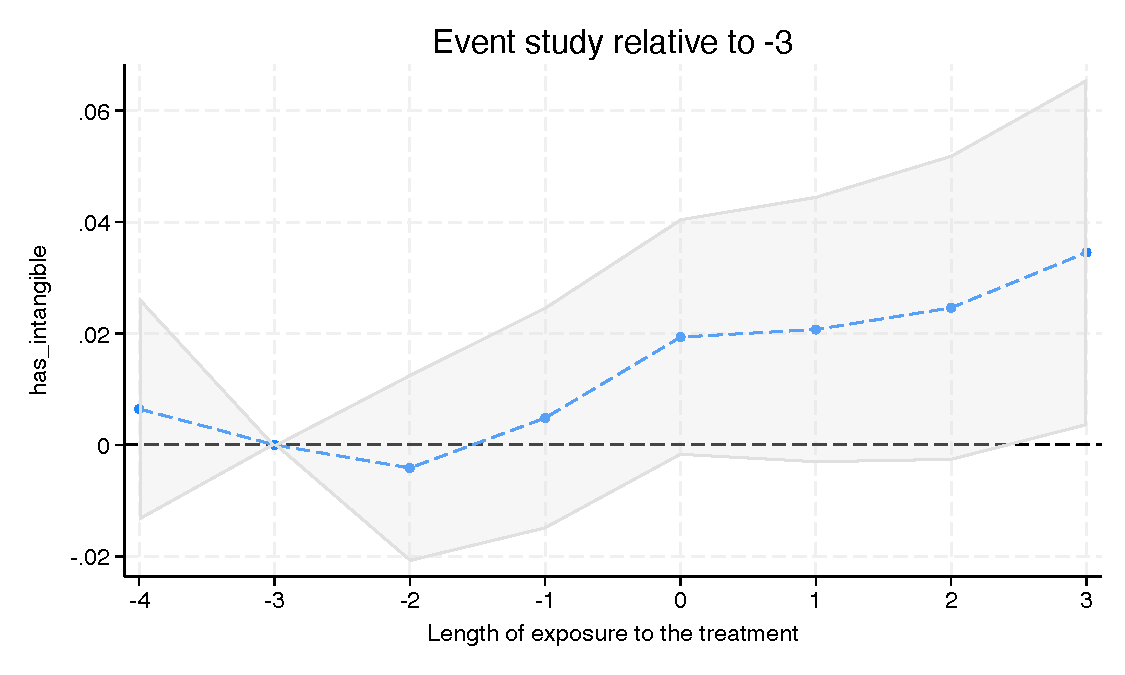
\includegraphics[width=0.8\textwidth]{figure/event_study_has_intangible.pdf}
\caption{Evolution of Intangible Assets Under Good vs Bad CEOs}
\label{fig:intangibles}
\end{figure}

The contrasting dynamics between materials and capital provide particularly compelling evidence for our framework. Figure \ref{fig:materials} shows that material purchases jump immediately by [[immediate materials jump]] percent in year 0 under good CEOs, consistent with managers having direct control over input purchases. Meanwhile, capital shows no discontinuous change at the transition point, confirming that physical investment remains under owner control.

\begin{figure}[htbp]
\centering
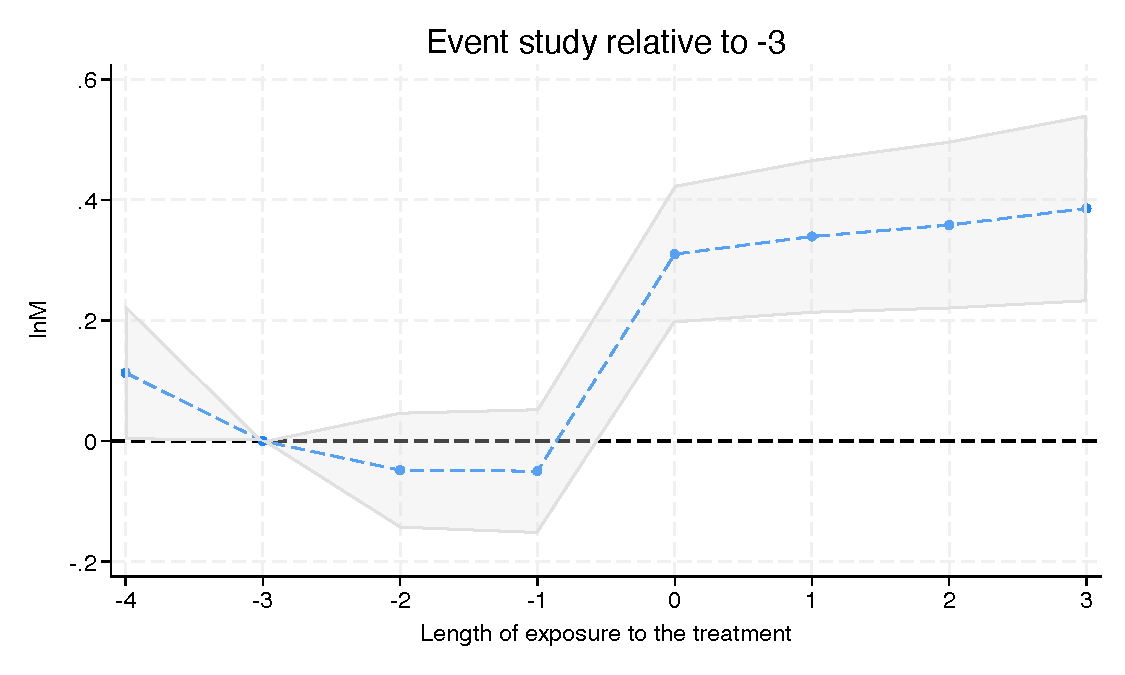
\includegraphics[width=0.8\textwidth]{figure/event_study_lnM.pdf}
\caption{Immediate Adjustment of Material Inputs Under New CEOs}
\label{fig:materials}
\end{figure}

These differential effects across outcomes—immediate for manager-controlled variables, gradual or absent for owner-controlled ones—support our model's division of decision rights and strengthen the causal interpretation of our estimates.

\section{Conclusion}

Our main finding is that three-quarters of the apparent CEO effect is spurious. The naive comparison of firms hiring good versus bad CEOs suggests a [[raw CEO gap]] percent performance difference. However, our placebo-controlled event study reveals that [[placebo gap]] percent of this gap arises from mechanical noise in fixed effects estimation. The true causal effect is only [[true CEO effect]] percent—a quarter of what raw correlations suggest.

CEOs matter modestly, with their primary impact coming through scaling variable inputs. Better managers expand operations by immediately increasing employment and material purchases, generating higher revenues within the constraints of owner-controlled capital. The [[true CEO effect]] percent productivity advantage translates into approximately [[revenue effect]] percent higher revenues through this scaling mechanism. The immediate response of manager-controlled variables contrasted with unchanged capital stocks validates our model's division of decision rights between owners and managers.

These findings have profound implications for corporate governance and productivity research. The widespread practice of using manager fixed effects as explanatory variables is fundamentally flawed—with [[percent noise]] percent noise contamination, such estimates suffer from severe attenuation bias. This explains the weak and inconsistent relationships often found in studies relating manager "quality" to firm policies or outcomes. Researchers should not trust raw CEO fixed effects as measures of managerial ability.

Instead, future research should use observable manager characteristics. Education and work experience \citep{DePirro2025}, foreign name as a proxy for international exposure \citep{Koren2023expat}, and the selectiveness of entry cohorts \citep{koren2024managers} offer more reliable, albeit narrower, measures of specific dimensions of managerial quality. These observables, while capturing only partial aspects of CEO ability, avoid the mechanical noise that contaminates fixed effects estimates.

Several open questions warrant further investigation. Our connected component covers only [[percent in component]] percent of managers, raising concerns about representativeness for the broader population of private firms. The high prevalence of founder-CEOs ([[percent founders]] percent) may mask heterogeneous effects between founders and professional managers. The transition economy period of the 1990s likely differs from the post-2004 EU membership era in terms of managerial practices and their impacts. Addressing these questions requires targeted sampling strategies and period-specific analyses that we leave for future work.

\bibliographystyle{apalike}
\bibliography{references}

\appendix

\section{Additional Tables and Figures}

[Appendix content to be added]

\end{document}
